\subsection{③}
  \begin{figure}[H]
    \begin{tabular}{ccc}
      \begin{minipage}{.5\textwidth}
        \centering
        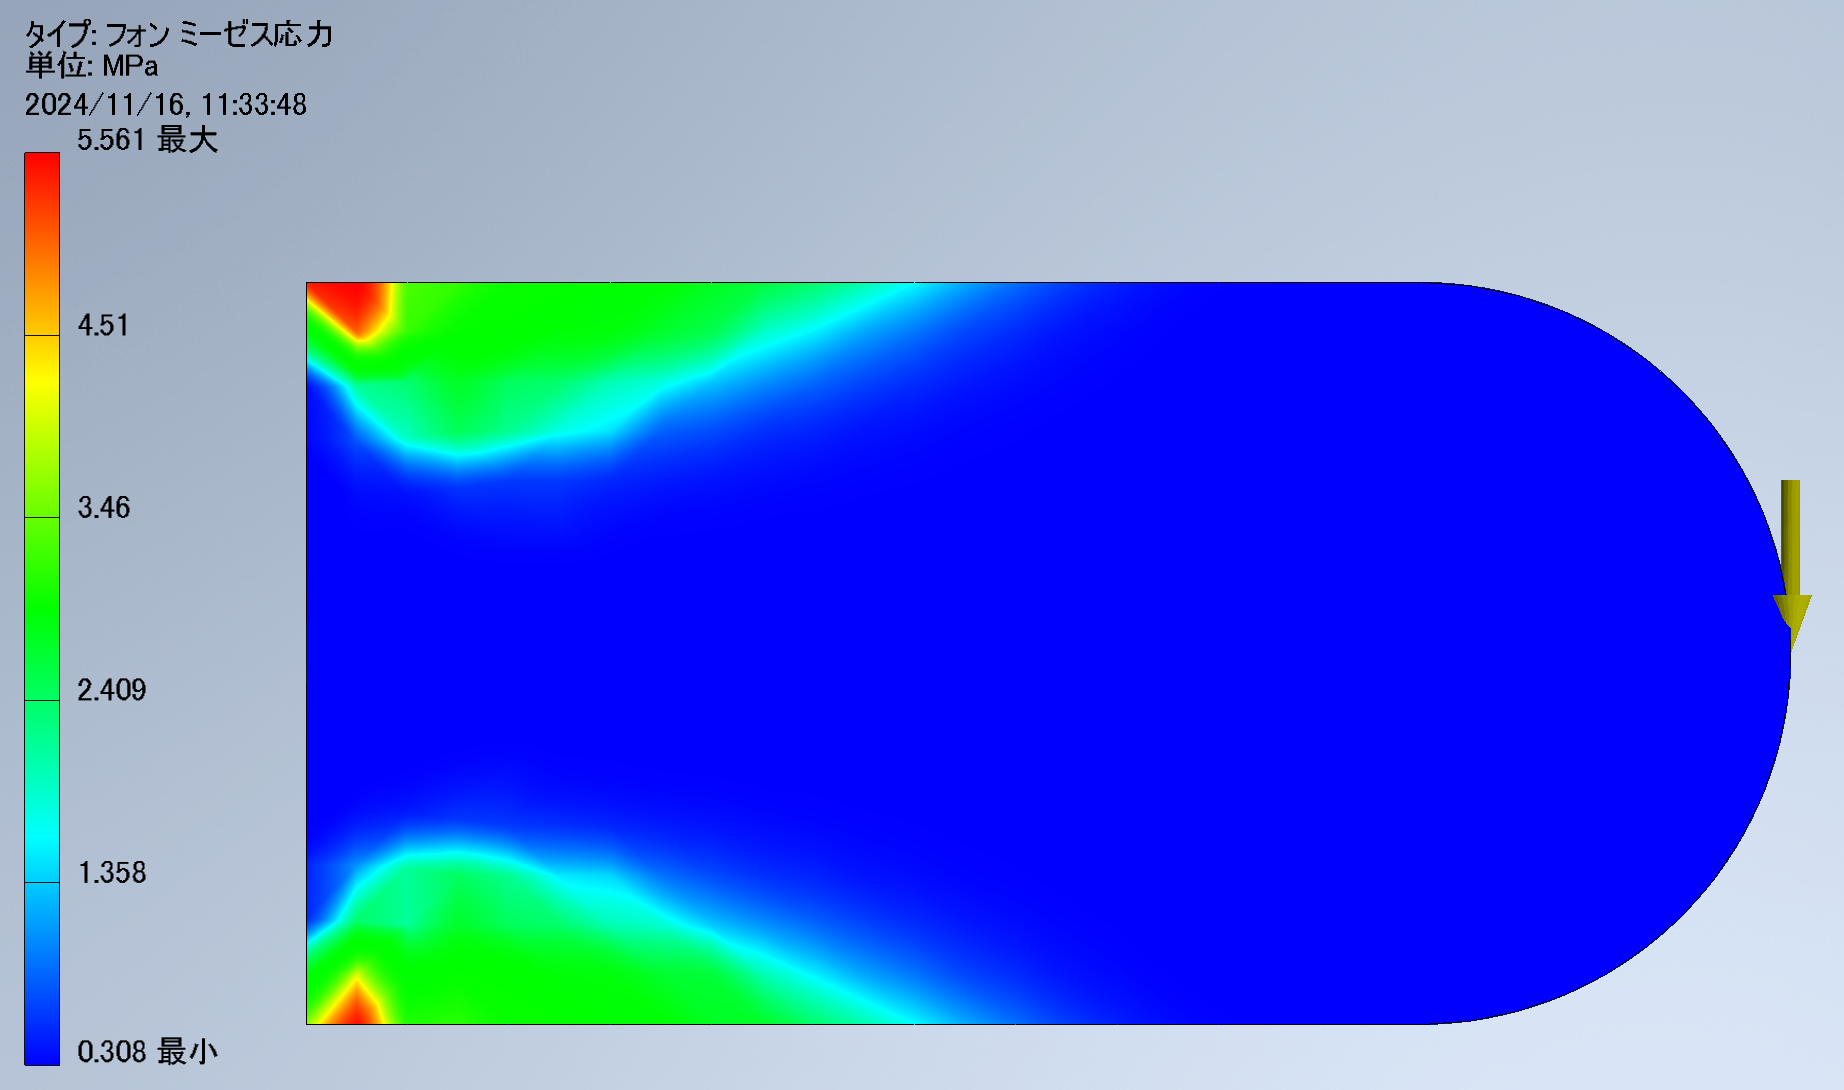
\includegraphics[width=0.99\linewidth]{images/3_voms.png}
        \caption{応力}
        \label{img:3_voms}
      \end{minipage}
      \begin{minipage}{.5\textwidth}
        \centering
        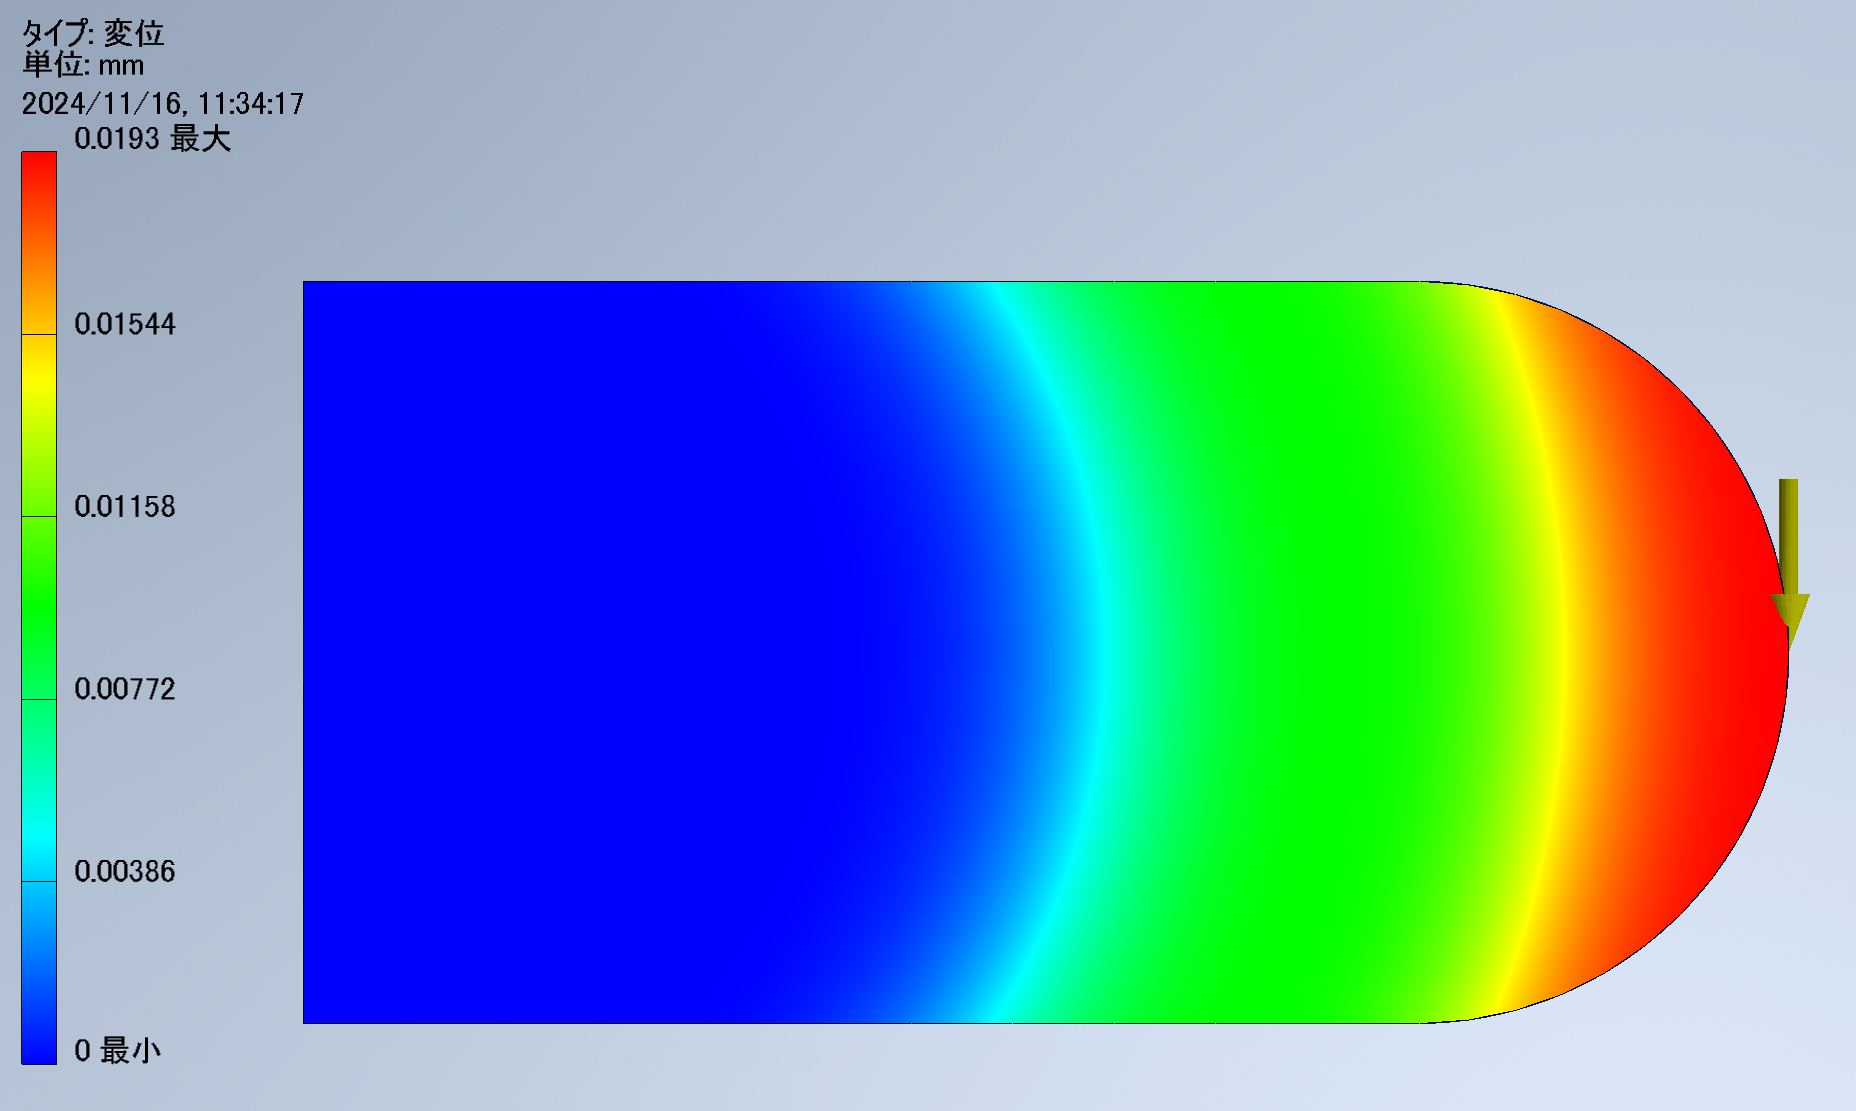
\includegraphics[width=0.99\linewidth]{images/3_disp.png}
        \caption{変位}
        \label{img:3_disp}
      \end{minipage}
    \end{tabular}
  \end{figure}

  以上の図は②で施したフィレットを左下の辺にも施し,実験を行った結果である.
  解析条件は以下.
  \begin{equation*}
    V \approx 47096[mm^3]
  \end{equation*}

  図\ref{img:3_voms}より集中荷重を加えている場所の応力を,
  ほぼ一様に分散することができていることがわかる.
  また応力の最大値も減少していることがわかる.
  図\ref{img:3_disp}より変位の分散の仕方は変わっていないが,
  変位の最小値が減少していることがわかる.\\\indent
  今回も体積が小さくなってしまったが,応力と変位を小さくすることができた.\\\indent
  次の実験は削った体積分を梁の補強に充てて行う.
